\section{Results}
\label{sec:results}

\subsection{Controlled impairments}

Figure~\ref{fig:impairments} and Table~\ref{tab:quantitative-results} report the main impairment results. The direct historical 20-Mbps record measured 19.2 Mbps, a $-4.00\%$ deviation, but supplies no SD or confidence interval. The supplementary 50-Mbps cohort measured 41.500 Mbps (SD 3.362, 95\% CI $\pm4.175$, range 36.9--45.8), a $-17.00\%$ deviation. At 100 Mbps the five valid measurements averaged 78.780 Mbps (SD 11.684, 95\% CI $\pm14.508$, range 58.4--87.3), a $-21.22\%$ deviation. These 50/100-Mbps statistics are repository-reported from the retained supplementary cohort. The dual-router 20-Mbps benchmark is excluded from this direct-topology panel.

\begin{figure}[t]
\centering
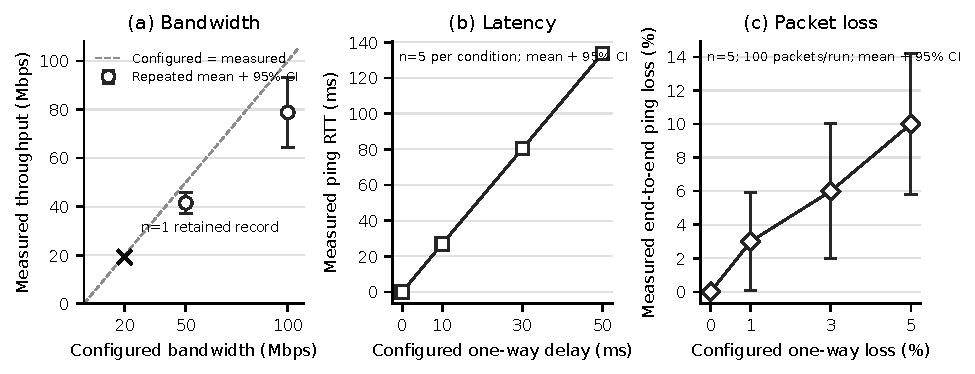
\includegraphics[width=\linewidth]{figures/bandwidth/main_impairment_results.pdf}
\caption{Main impairment results. Bandwidth distinguishes the single historical 20-Mbps record from replicated 50/100-Mbps cohorts. Latency plots configured one-way delay against measured ping RTT. Packet loss plots configured one-way loss against measured end-to-end ping loss. Error bars are shown only for repeated cohorts and represent 95\% confidence intervals.}
\label{fig:impairments}
\end{figure}

\begin{table}[t]
\caption{Main impairment results. BW denotes bandwidth; CI denotes the 95\% confidence-interval half-width; RR and AC denote repository-reported and audit-computed values.}
\label{tab:quantitative-results}
\centering
\setlength{\tabcolsep}{2.5pt}
\begin{tabular}{lrrrrrl}
\hline
Condition & $n$ & Mean & SD & 95\% CI & Range & Deviation/source \\
\hline
BW 20 Mbps & 5 & 19.200 & 0.000 & $\pm0.000$ & 19.200--19.200 & $-4.00\%$; RR \\
BW 50 Mbps & 5 & 47.800 & 0.100 & $\pm0.124$ & 47.700--47.900 & $-4.40\%$; RR \\
BW 100 Mbps & 5 & 94.760 & 0.913 & $\pm1.133$ & 93.200--95.500 & $-5.24\%$; RR \\
Delay 0 ms & 5 & 0.105 & 0.019 & $\pm0.024$ & 0.080--0.123 & RTT; RR/AC \\
Delay 10 ms & 5 & 27.008 & 0.056 & $\pm0.070$ & 26.943--27.089 & RTT; RR/AC \\
Delay 30 ms & 5 & 80.303 & 0.057 & $\pm0.071$ & 80.249--80.393 & RTT; RR/AC \\
Delay 50 ms & 5 & 133.686 & 0.037 & $\pm0.046$ & 133.637--133.723 & RTT; RR/AC \\
Loss 0\% & 5 & 0.000 & 0.000 & $\pm0.000$ & 0--0 & end-to-end; RR/AC \\
Loss 1\% & 5 & 3.000 & 2.345 & $\pm2.912$ & 1--7 & end-to-end; RR/AC \\
Loss 3\% & 5 & 6.000 & 3.240 & $\pm4.023$ & 2--9 & end-to-end; RR/AC \\
Loss 5\% & 5 & 10.000 & 3.391 & $\pm4.211$ & 5--14 & end-to-end; RR/AC \\
\hline
\end{tabular}
\vspace{1mm}

\raggedright Bandwidth uses one fixed-block session ($n=5$ per rate); its intervals are descriptive and older cohorts are not pooled. Units are Mbps for bandwidth, ms for RTT, and percent for loss.
\end{table}


Mean RTT increased from 0.105 ms at 0-ms configured one-way delay to 27.008, 80.303, and 133.686 ms at 10, 30, and 50 ms. The corresponding AC sample SDs were 0.019, 0.056, 0.057, and 0.037 ms, with CI half-widths 0.024, 0.070, 0.071, and 0.046 ms. The means are RR; SD, CI, minimum, and maximum values in Table~\ref{tab:quantitative-results} are AC. These observations are RTTs and are not reported as measured one-way latency.

Configured one-way loss of 0, 1, 3, and 5\% produced RR mean end-to-end ping loss of 0, 3, 6, and 10\%. Across five runs per condition, the AC SDs were 0, 2.345, 3.240, and 3.391 percentage points; confidence intervals widened accordingly. Aggregate packet counts were 500/500, 485/500, 470/500, and 450/500 received/sent. Because impairment configuration and ping observation cover different directions and constructs, no direct relative-error statistic is assigned.

The separate dual-router benchmark completed five valid runs with a mean throughput of 19.220 Mbps, SD 0.045, 95\% CI $\pm0.056$, and range 19.2--19.3 Mbps. The mean is RR; dispersion and range are AC.

\subsection{Topology scaling and Germany50}

Figure~\ref{fig:topology-scaling} separates simple execution, the dual-router benchmark, and full Germany50 scope. In the controlled extracted-path experiments, the one-hop shortest path produced mean RTT 41.196 ms (AC SD 0.259, CI $\pm0.642$) and mean throughput 18.8 Mbps. The four-hop median path produced 104.623 ms (SD 0.845, CI $\pm2.098$) and 17.8 Mbps. The nine-hop longest path produced 214.425 ms (SD 0.441, CI $\pm1.095$) and 15.7 Mbps. Relative to 20 Mbps, the reported throughput deviations were $-6.0\%$, $-11.0\%$, and $-21.5\%$.

\begin{figure}[t]
\centering
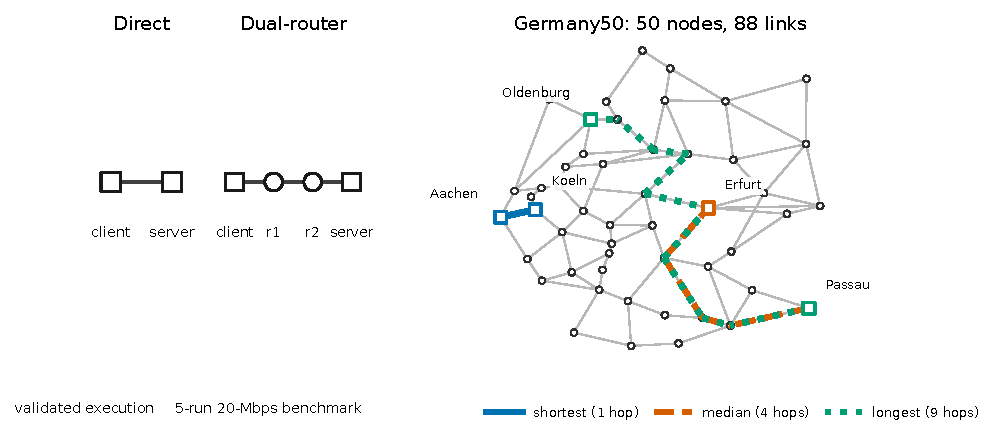
\includegraphics[width=\linewidth]{figures/germany50/topology_scaling_germany50.pdf}
\caption{Topology scaling from direct and dual-router configurations to the real 50-node/88-link Germany50 graph. Highlighted paths are the shortest, median, and longest representative paths used for real traffic. The 4,224-entry full route plan was validated in dry-run mode only; the figure does not represent all-pairs traffic.}
\label{fig:topology-scaling}
\end{figure}

The full topology preflight recorded 50 nodes, 88 networks, and a theoretical 4,224-route plan. Selected mode installed 20 routes and completed three ping/iperf3 measurements for each representative pair (nine total). The full 4,224-entry plan separately returned dry-run success. No retained evidence shows that all entries were installed or that all node pairs exchanged real traffic.

\subsection{AI, closed-loop control, and Dashboard}

Table~\ref{tab:extended-validation} summarizes the extensions. The official OpenAI attempt returned HTTP 429 with \texttt{insufficient\_quota}; it generated no successful official scenario. The separate Qwen-compatible request produced a validated scenario and a single controlled real-Docker result of 82.194-ms RTT, 18.3-Mbps throughput, and 0\% measured loss. No SD or CI is available for this single validation.

\begin{table}[t]
\caption{Extended validation and evidence boundaries.}
\label{tab:extended-validation}
\centering
\setlength{\tabcolsep}{1.5pt}
\begin{tabular}{p{0.13\linewidth}p{0.22\linewidth}p{0.28\linewidth}p{0.33\linewidth}}
\hline
Component & Evidence & Result & Boundary \\
\hline
Dual-router & Five Docker runs & 19.220 Mbps mean; SD 0.045; CI $\pm0.056$ & Separate multi-router benchmark; not part of a direct cohort. \\
Germany50 & Full instantiation; route summaries; nine measurements & 50 nodes/88 links; 4,224-entry plan passed dry-run; three paths carried traffic & Dry-run is not route installation; traffic was representative, not all-pairs. \\
AI & Sanitized official result; compatible-provider run & Official OpenAI: HTTP 429. Qwen-compatible: validated success & Providers remain separate; Qwen success is not official OpenAI success. \\
RL & Per-episode CSV; policy summary & 80 valid Docker measurement rows; mean reward 17.116 heuristic vs 4.143 Q-learning & Higher heuristic mean applies only to the evaluated setup. \\
Dashboard & Validation document; implementation & Documented smoke: 0.118-ms mean RTT; 19.4 Mbps & Raw UI/test/security/secret/fresh-clone logs were not retained. \\
\hline
\end{tabular}
\end{table}


Across the balanced RL supplement, the threshold heuristic achieved RR mean reward 17.116 (SD 0.325, 95\% CI $\pm0.142$), mean RTT 30.189 ms, 0\% mean loss, and 18.625-Mbps mean throughput. Q-learning achieved mean reward 4.143 (SD 15.045, CI $\pm6.594$), mean RTT 89.225 ms, 2.5\% loss, and 9.855-Mbps throughput. AC reward ranges were 16.615--17.471 for the heuristic and $-36.975$--17.472 for Q-learning. Q-learning selected path A in all 20 episodes and made no switch; the heuristic selected A for ten episodes, B for ten, and switched once at the phase boundary.

\begin{figure}[t]
\centering
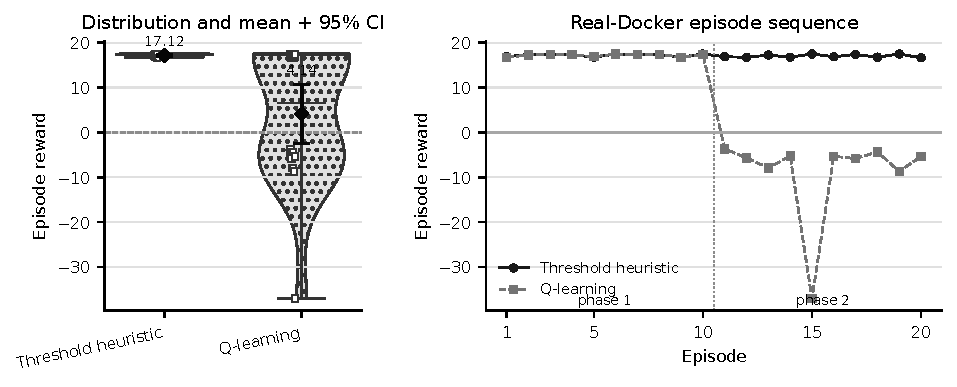
\includegraphics[width=\linewidth]{figures/rl/rl_heuristic_vs_qlearning.pdf}
\caption{Reward comparison for the 20 valid real-Docker episodes of each displayed policy. The complete retained supplement contains 80 valid episodes across Q-learning, threshold heuristic, fixed A, and fixed B. Both the distribution and episode sequence show that the threshold heuristic materially outperformed Q-learning under the evaluated setup.}
\label{fig:rl}
\end{figure}

The Dashboard validation document records direct run \texttt{3cada000bb4d}: three of three ping replies, RTT min/mean/max 0.101/0.118/0.143 ms, 19.4-Mbps throughput, HTTP 200 for JSON/CSV/log/ZIP downloads, and cleanup pass. The raw UI-run, 69-test, security, secret-scan, and fresh-clone logs are not retained, so this result remains documented-only.
